\chapter{Analysis Of Existing}

As said before, drone swarm are governed by these models mobility. Our study of the existing is therefore divided into several parts.

\section{Summary of the problem}

The issue of this paper is to scan an area as efficiently as possible and as quickly as possible, at least once per hour. This area will be scanned by a UAV swarm that will cooperate and communicate each other.

\section{Existing models}

Many mobility models exist with different characteristics. All these models are used to define movements for swarm of UAV. Most models are based on real-life situations such as road maps, or on the behavior of many animals (ants, birds, termites, wolves etc). We will expose some of them we consider the most important and most interesting for our case.

\subsection{Random Walk}

First described by Einstein in 1926, it was developed to mimic the extremely unpredictable movement of many entities in nature. An mobility node (MN) moves from its position to a new one by randomly choosing a direction and speed chosen by pre-defined ranges, [speedmin, speedmax] and [0, 2PI]. At the end of a constant time interval t or a constant distance traveled d, a new speed and direction are calculated. If a MN during his travel reaches a simulation boundary, it « bounces » off the simulation border with an angle determined by the incoming direction and continues to this new path.
It's a memory-less mobility pattern because it retains no knowledge of its old locations and speed values. Therefore, the current position and speed of a MN is independent of its past location and speed. This can generate unrealistic movement because of sudden stops and sharp turns. If the specified time or distance of a MN motion is short, the resulting movement pattern will be a random roaming pattern restricted to a small part of the simulation area. The Figure \ref{RandomWalk} shows an example of the movement observed from this model. All the MN begin in the center of the 300mx600m simulation area (at the position (150,300)). Every 60 seconds, each MN randomly choose a direction between 0 and 2PI, and a speed between 0 and 10m/s.

\begin{figure}[h]
\center
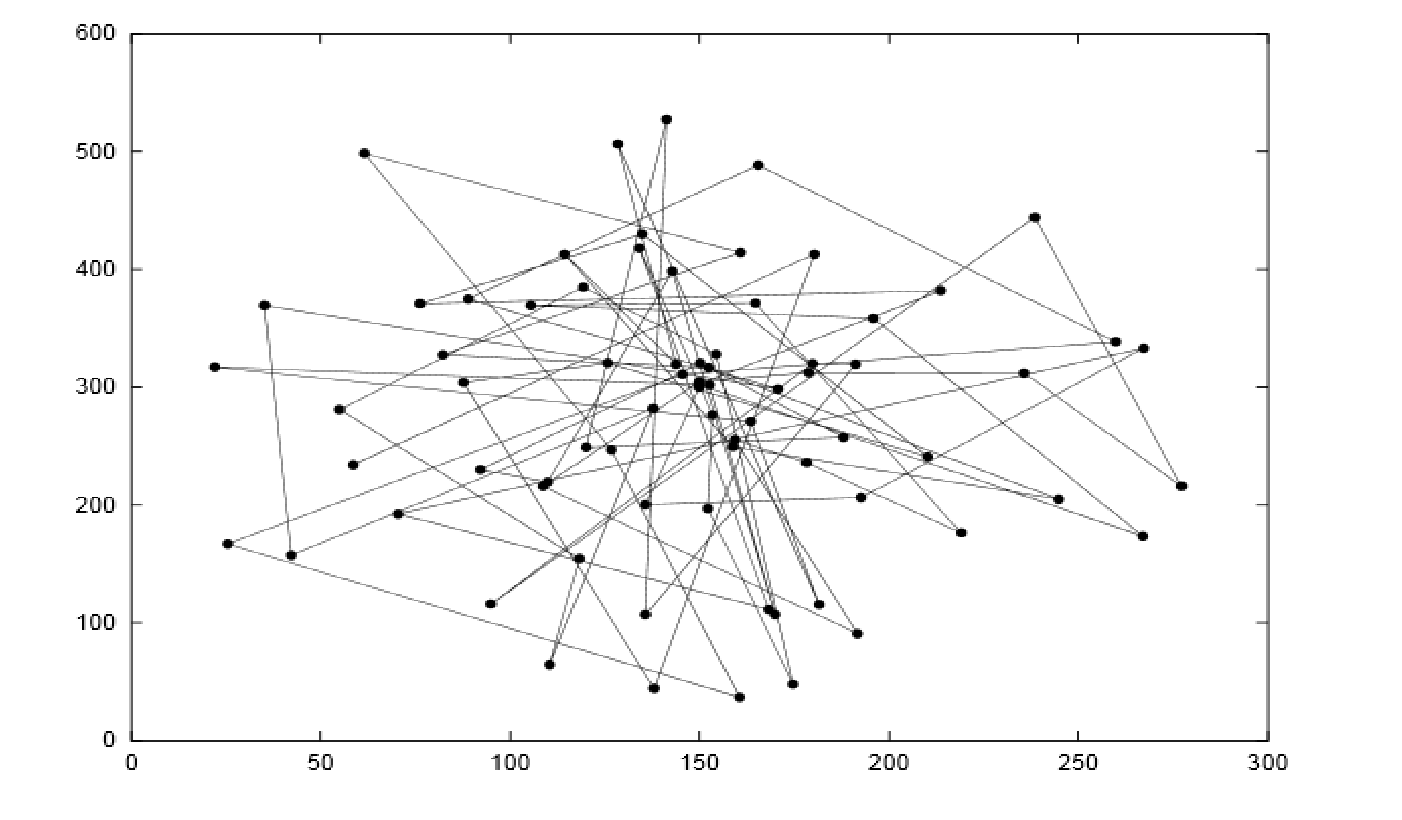
\includegraphics[width=7cm,height=50mm]{../images/randomwalk1.png}
\caption{\label{RandomWalkFig}Resulting pattern of a MN using the Random Walk Mobility Model}
\end{figure}


\textbf{METTRE DES SCHEMA ET DECRIRE PLUS...et maintenant?}

\subsection{Random Waypoint}

Includes pause times between changes in direction and/or speed.Once this time expires, the MN chooses a random destination and a speed, that is uniformly distributed between [minspeed, maxspeed]. The movement pattern of a MN who uses the RWaypointMM is similar to the RWalkMM if pause time is zero and [minspeed, maxspeed] = [speedmin, speedmax]. The Figure \ref{RandomWaypointFig} shows an example of the resulting pattern from the Random Waypoint Mobility Model.

\begin{figure}[h]
\center
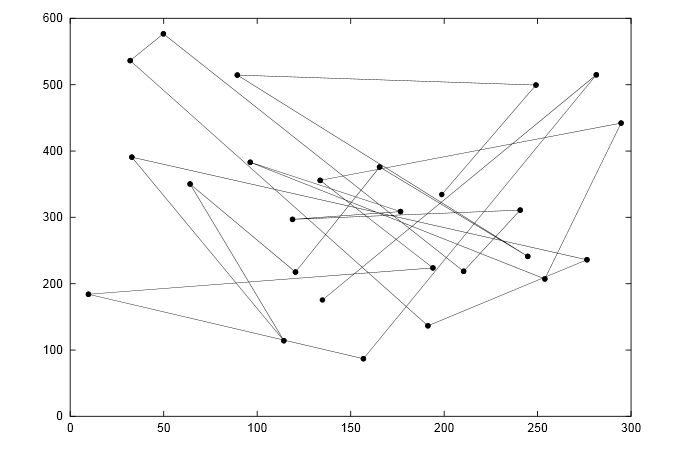
\includegraphics[width=7cm,height=50mm]{../images/randomwaypoint1.png}
\caption{\label{RandomWaypointFig}Resulting pattern of a MN using the Random Waypoint Mobility Model}
\end{figure}

During a run, MNs are initially distributed randomly around the simulation area. Figure \ref{RandomWaypointFig2} shows the average MN neighbor percentage of the MNs. For example, if there are 50 MNs in the network and a node has 10 neighbors, then the node's current neighbor percentage is 20\%. Moreover, during the first 600 seconds, due to initially distributed randomly of the MNs around the simulation area, there is an high variability in the average MN neighbor percentage.
In the paper, there is presented three possible solutions to avoid this initialization problem. The first is to save the location of the MNs after the initial high variability and use this position as the initial starting point of the MNs in all future simulations. Second, initially distribute the MNs in a specific area to be a distribution more common the model, like fore example, initially placing the MNs in a triangle distribution. Lastly, discard the initial 1000 seconds of simulation time in each simulation trials, to ensure that the initialization problem is removed even if the MNs move slowly. But if the MNs move fastly, we can discard fewer seconds of simulation time. This third solution ensures that each simulation has a random initial configuration.
Figure 5 : there is a complex relationship between node speed and pause time. A scenario with fast MNs and long pause times actually produces a more stable networks than a scenario with slower MNs and shorter pause times. Hence, long pause times(over 20 seconds) produce a stable network even at high speeds.

\begin{figure}[h]
\center
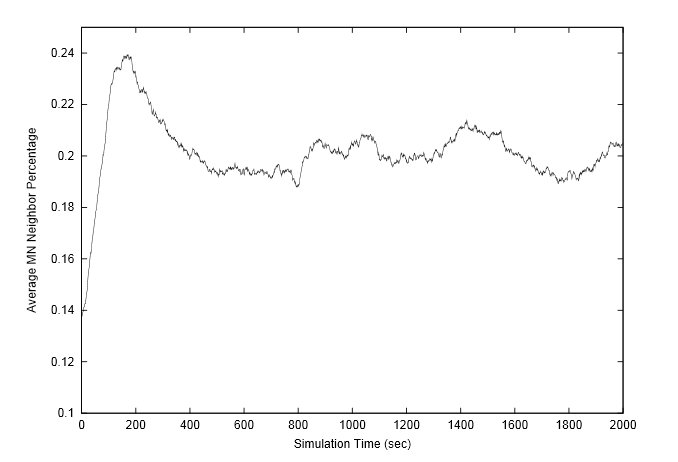
\includegraphics[width=7cm,height=50mm]{../images/randomwaypoint2.png}
\caption{\label{RandomWaypointFig2}Average neighbor percentage vs. time}
\end{figure}

\textbf{METTRE DES SCHEMA ET a revoir}

\subsection{City section}

The aim of this model is to propose a realistic model. It bases on the vehicle's movement on road maps. The specificity of this model is the map depends on each geographical zone. Here, vehicles are mobile nodes.\\\\

The mapping data blocks are available from the office Americans of the census. The map information is retrieved from text files. These files are composed of several elements:

\begin{itemize}
\item The unique identifier for a specified road.
\item The nature of the road: it can be a highway or a street.
\item The longitude of the start of position.
\item The latitude of the start of departure
\item The latitude of arrived.
\item The longitude of arrived.
\end{itemize}

All the intersections of the map are represented by nodes not mobile.
This model also considers the volume of traffic : more traffic, the more the line representing the road will be thick.
This model is also sensitive at the speed of cars (depending in particular on the hour). For example, we can consider that the speed of vehicular traffic in the morning is much smaller than at the beginning of the afternoon.\\\\

Here is the progress of this model. Every node begins in a point chosen randomly and its destination is chosen also randomly. The strategy of every node is to look for the shortest way until the destination. To achieve it, the algorithm of Dijkstra is used. Several parameters has to be considered in this algorithm as the speed or the traffic. This route can be dynamically changed. When a node reachs its destination, it begins again all the process described previously. Concerning the node's speed, it is limited to more or less 5\% of the speed registered in the file.\\
For example, here is a representation of the model. We see here that the traffic is little sparse, but with very different speeds.

\begin{figure}[h]
\center
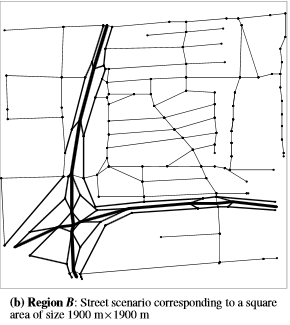
\includegraphics[width=7cm,height=50mm]{../images/city.png}
\caption{City application}
\end{figure}

\textbf{METTRE DES SCHEMA ET a compléter}

\subsection{Natural Agent}

\subsubsection{Ants}

Le modèle de mobilité des fourmis se base sur le fait que les fourmis construisent des réseaux de sentiers qui relient leurs   nids avec des sources de nourritures disponible.
Chaque fourmi qui se nourrit à le même programme :

\begin{itemize}
\item Elle doit éviter les obstacles.
\item Aller ou elle veut (déplacement aléatoire) tant qu'il n'y a pas de phéromones.
\item Si elle arrive à trouver de la nourriture, elle laisse des phéromones pendant un temps t pour pouvoir indiquer aux autres fourmis l'emplacement de la nourriture.
\item Si la fourmi trouve de la nourriture, elle l'a ramène à son nid.
\end{itemize}

Les fourmis peuvent mourir. Soit elles ne trouvent pas de la nourriture assez rapidement et meurt de faim, soit elles se font tuer par d'autres prédateurs.
Tous les chemins de phéromones conduisent à de la nourriture. Mais les phéromones s'évaporent dans le temps. Le taux de phéromone peut être renforcé si plusieurs fourmis passent par le même chemin.

\textbf{METTRE DES SCHEMA ET a compléter}

\subsubsection{Termites}

\subsubsection{Wasps}

le modèle basé sur les guêpes est composé de plusieurs caractéristiques :
\begin{itemize}
\item un chef qui répartit les différentes guêpes dans différents groupes
\item 
\end{itemize}

\subsection{Birds and Fish}

\subsection{Wolves}
